\documentclass[aspectratio=169]{beamer}
%
% Choose how your presentation looks.
%
% For more themes, color themes and font themes, see:
% http://deic.uab.es/~iblanes/beamer_gallery/index_by_theme.html
%
\mode<presentation>
{
  \usetheme{metropolis}      % or try Darmstadt, Madrid, Warsaw, ...
  \usecolortheme{metropolis-imagelab} % or try albatross, beaver, crane, ...
  \usefonttheme{structurebold}  % or try serif, structurebold, ...
  \setbeamercolor{background canvas}{bg=white}
  \setbeamertemplate{navigation symbols}{}
  \setbeamertemplate{bibliography item}{\insertbiblabel}
  %\setbeamertemplate{caption}[numbered]
} 
\usepackage[english]{babel}
\usepackage[utf8x]{inputenc}
\usepackage{hyperref}
\usepackage{algorithm,algorithmic}
\usepackage{multirow}
\usepackage{pifont}% http://ctan.org/pkg/pifont
\newcommand{\cmark}{\ding{51}}%
\newcommand{\xmark}{\ding{55}}%

\usepackage{listings}             % Include the listings-package
\usepackage{pgfplots}
\usepackage{caption}
\usepackage{xcolor}
\usepackage{amsmath}

\usepackage{tikz}
\usepackage{animate}
\usepackage{bm}


\hypersetup{
    colorlinks = true,
    linkcolor = {black},
    urlcolor = {mImagelabRed}
}

\DeclareMathOperator*{\argmin}{arg\,min}
\DeclareMathOperator*{\argmax}{arg\,max}
\newcommand{\highlight}[1]{\textcolor{mImagelabRed}{#1}}

\title[Reinforcement Learning]{Reinforcement Learning}
\subtitle{Function approximation}
\institute{University of Modena and Reggio Emilia}
\author{Davide Abati}
\date{\today}

\def\thisframelogos{}

\newcommand{\framelogo}[1]{\def\thisframelogos{#1}}
%\algnewcommand{\myRepeat}[1]{\State \algorithmicrepeat \unskip #1}

\begin{document}

\framelogo{logo_unimore_white.png}

\bgroup
\renewcommand{\insertframenumber}{}
\begin{frame}[noframenumbering]
  \titlepage
\end{frame}
\egroup
\bgroup
\begin{frame}{Disclaimer}
All this material is a free re-arrangement of \href{http://www0.cs.ucl.ac.uk/staff/d.silver/web/Teaching.html}{David Silver's UCL Course on RL}.
\\
You are also encouraged to take a look to his \href{https://www.youtube.com/watch?v=2pWv7GOvuf0}{Youtube lectures}.
\end{frame}
\egroup

\section*{Introduction}
\bgroup
\begin{frame}{Large scale reinforcement learning}
Reinforcement learning can be used to solve large problems, e.g.
\begin{itemize}
\item Backgammon: $10^{20}$ states
\item Computer Go: $10^{170}$ states
\item Helicopter: continuous state space
\end{itemize}
\onslide<2->{
How can we scale up the model-free methods for prediction and control from the last lecture?}
\end{frame}
\egroup
\bgroup
\begin{frame}{Value function approximation}
\begin{itemize}
\item So far we have represented value function by a lookup table
\begin{itemize}
\item Every state $s$ has an entry $V(s)$
\item Or every state-action pair $s, a$ has an entry $Q(s, a)$
\end{itemize}
%
\item Problem with large state spaces:
\begin{itemize}
\item There are too many states and/or actions to store in memory
\item It is too slow to learn the value of each state individually
\end{itemize}
%
\item Solution for large state spaces:
\begin{itemize}
\item Estimate value function with function approximation
\begin{align*}
\hat{v}(s,\textbf{w}) &\approx v_{\pi}(s)\\
\hat{q}(s, a, \textbf{w}) &\approx q_{\pi}(s, a)
\end{align*}
\item Generalise from seen states to unseen states
\item Update parameter $w$ using MC or TD learning
\end{itemize}
\end{itemize}
\end{frame}
\egroup
\bgroup
\begin{frame}{Types of value function approximation}
\begin{figure}
\centering
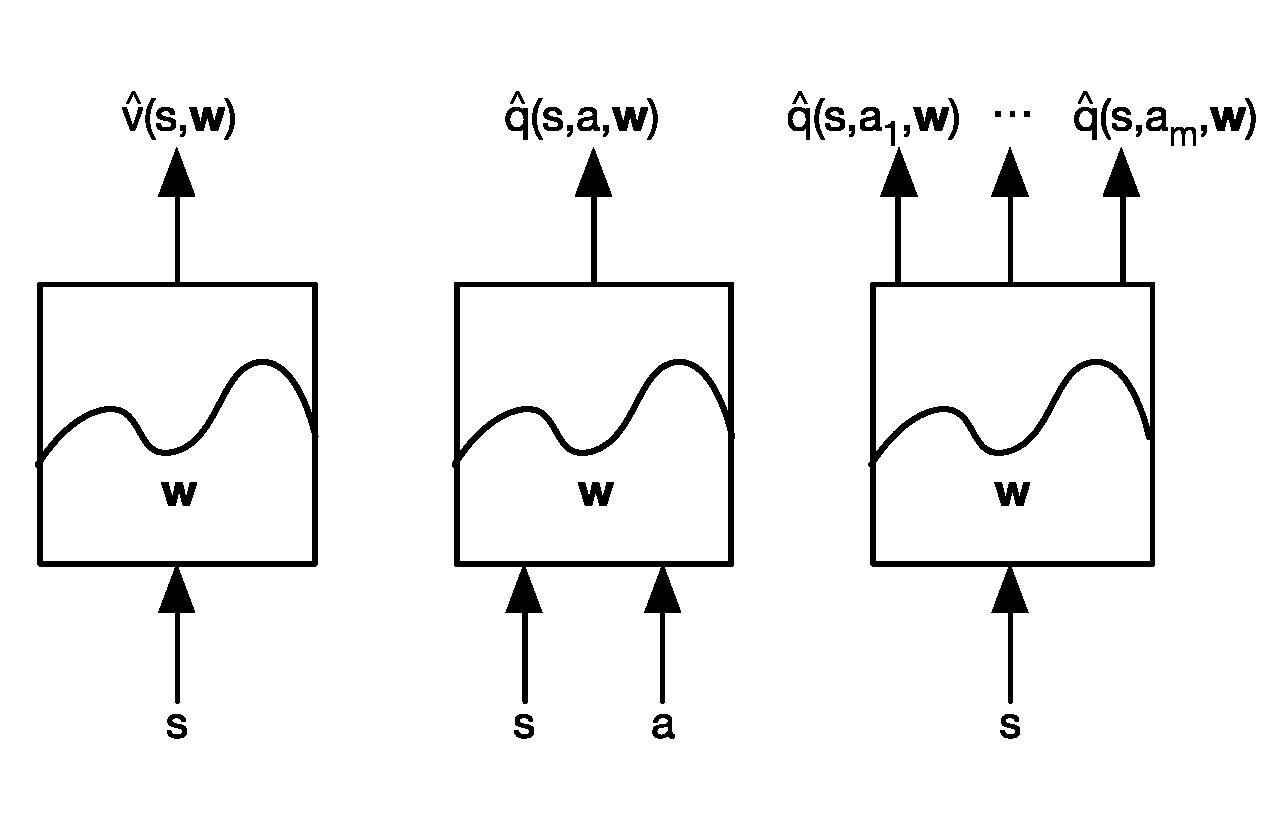
\includegraphics[width=0.8\textwidth]{img/vfa_types.pdf}
\end{figure}
\end{frame}
\egroup
\bgroup
\begin{frame}{Which function approximator?}
There are many function approximators, e.g.
\begin{itemize}
\item Linear combinations of features
\item Neural network
\item Decision tree
\item Nearest neighbour
\item Fourier / wavelet bases
\item \ldots
\end{itemize}
\end{frame}
\egroup
\bgroup
\begin{frame}{Which function approximator?}
We consider \highlight{differentiable} function approximators, e.g.\begin{itemize}
\item \highlight{Linear combinations of features}
\item \highlight{Neural network}
\item Decision tree
\item Nearest neighbour
\item Fourier / wavelet bases
\item \ldots
\end{itemize}
Furthermore, we require a training method that is suitable for \highlight{non-stationary, non-iid} data
\end{frame}
\egroup

\section{Incremental methods}
\documentclass[aspectratio=169]{beamer}
\mode<presentation>
{
  \usetheme{metropolis}      % or try Darmstadt, Madrid, Warsaw, ...
  \usecolortheme{default} % or try albatross, beaver, crane, ...
  \usefonttheme{structurebold}  % or try serif, structurebold, ...
  \setbeamercolor{background canvas}{bg=white}
  \setbeamertemplate{navigation symbols}{}
  \setbeamertemplate{bibliography item}{\insertbiblabel}
  %\setbeamertemplate{caption}[numbered]
} 
\usepackage[english]{babel}
\usepackage[utf8x]{inputenc}
\usepackage{listings}             % Include the listings-package
\hypersetup{
    colorlinks = true,
    linkcolor = {black},
    urlcolor = {blue}
}
\usepackage{animate}
\usepackage{bm}

\setbeamertemplate{caption}{\raggedright\insertcaption\par}


\DeclareMathOperator*{\argmin}{arg\,min}

\title[Deep Learning and Temporal Data Processing]{Deep Learning and Temporal Data Processing}
\subtitle{0 - Gradient Descent}
\institute{University of Modena and Reggio Emilia}
\author{Andrea Palazzi}
\date{July 10th, 2017}

\def\thisframelogos{}

\newcommand{\framelogo}[1]{\def\thisframelogos{#1}}

\addtobeamertemplate{frametitle}{}{%
\begin{tikzpicture}[remember picture,overlay]
\node[anchor=north east] at (current page.north east) {%
    \foreach \img in \thisframelogos {%
        %\hspace{.5ex}%
        \includegraphics[height=3.5ex]{\img}%
    }%
};
\end{tikzpicture}}

\begin{document}

\framelogo{img/template/logo_unimore_white.png}

\bgroup
\renewcommand{\insertframenumber}{}
\begin{frame}[noframenumbering]
  \titlepage
\end{frame}
\egroup
\begin{frame}{Agenda}
  \tableofcontents
\end{frame}



%%%%%%%%%%%%%%%%%%%%%%%%%%%%%%%%%%%%%%%%%%%%%%%%%%%%%%%%%%%%%%%%%%
%%%%%%%%%%%%%%%%%%%%%%%%%%%%%%%%%%%%%%%%%%%%%%%%%%%%%%%%%%%%%%%%%%
%%%%%%%%%%%%%%%%%%%%%%%%%%%%%%%%%%%%%%%%%%%%%%%%%%%%%%%%%%%%%%%%%%


\section{Gradient Descent}

\begin{frame}{Gradient Descent}
\textbf{Gradient descent} is an iterative optimization algorithm for finding the minimum of a function. How? Take step proportional to the negative of the gradient of the function at the current point.
\begin{figure}
\begin{tabular}{c}
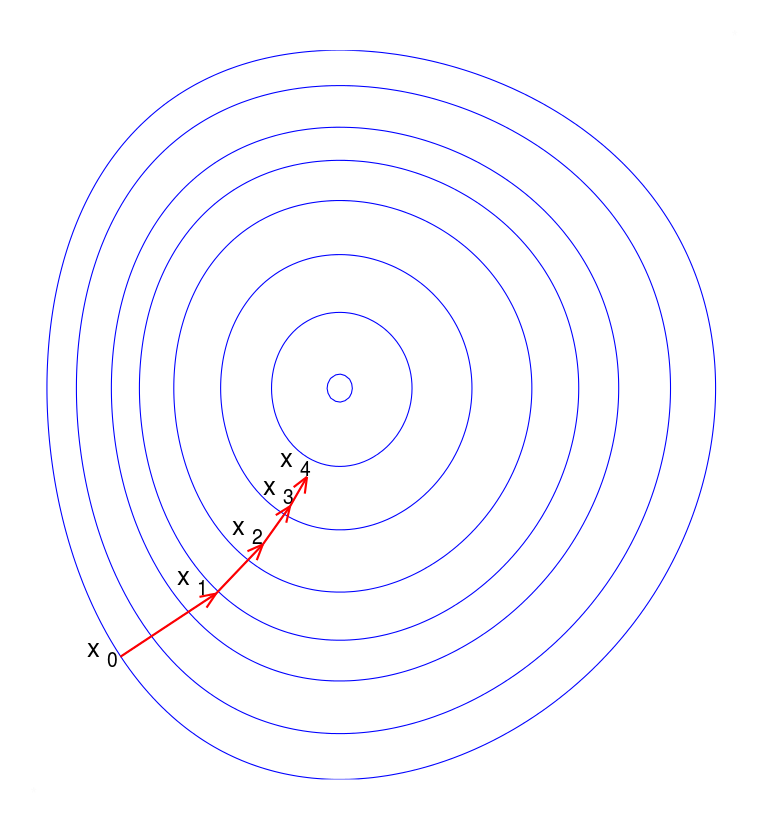
\includegraphics[width=0.3\textwidth]{img/sgd/level_sets.png}
\end{tabular}
\caption{Gradient descent on a series of level sets}
\end{figure}
\end{frame}

\begin{frame}{Gradient Descent Update}
If we consider a function $f(\bm{\theta})$, the \textbf{gradient descent update} can be expressed as:
\begin{equation}
\theta_j := \theta_j - \alpha \frac{\partial}{\partial \theta_j} f(\bm{\theta})
\end{equation}
for each parameter $\theta_j$.\\
\vspace{0.5cm}
The size of the step is controlled by \textbf{learning rate} $\alpha$.
\end{frame}

%%%%%%%%%%%%%%%%%%%%%%%%%%%%%%%%%%%%%%%%%%%%%%%%%%%%%%%%%%%%%%%%%%

%%%%%%%%%%%%%%%%%%%%%%%%%%%%%%%%%%%%%%%%%%%%%%%%%%%%%%%%%%%%%%%%%%

\begin{frame}{Visualizing Gradient Descent}
\begin{figure}
\begin{tabular}{c}
Gradient Descent for 1-d function $f(\theta)$.\\
  \animategraphics[loop,controls,width=0.9\textwidth]{1}{img/sgd/descent/descent-}{0}{7}
\end{tabular}
\end{figure}
\end{frame}


%%%%%%%%%%%%%%%%%%%%%%%%%%%%%%%%%%%%%%%%%%%%%%%%%%%%%%%%%%%%%%%%%%

\begin{frame}{Convexity}
Turns out that if the function is \textbf{convex} gradient descent will converge to the \textbf{global minimum}. For \textbf{non-convex} functions, it may converge to \textbf{local minima}.
\begin{figure}
\begin{tabular}{cc}
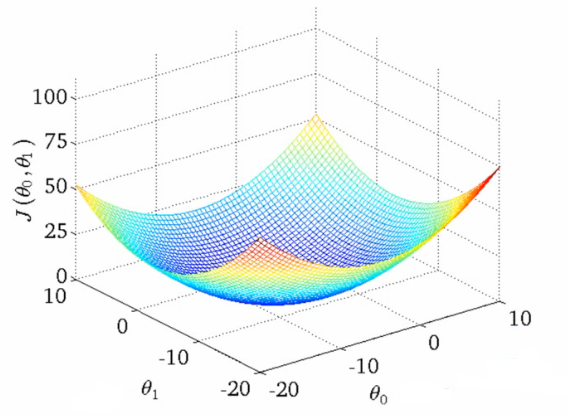
\includegraphics[width=0.4\textwidth]{img/sgd/convex_function.png} &
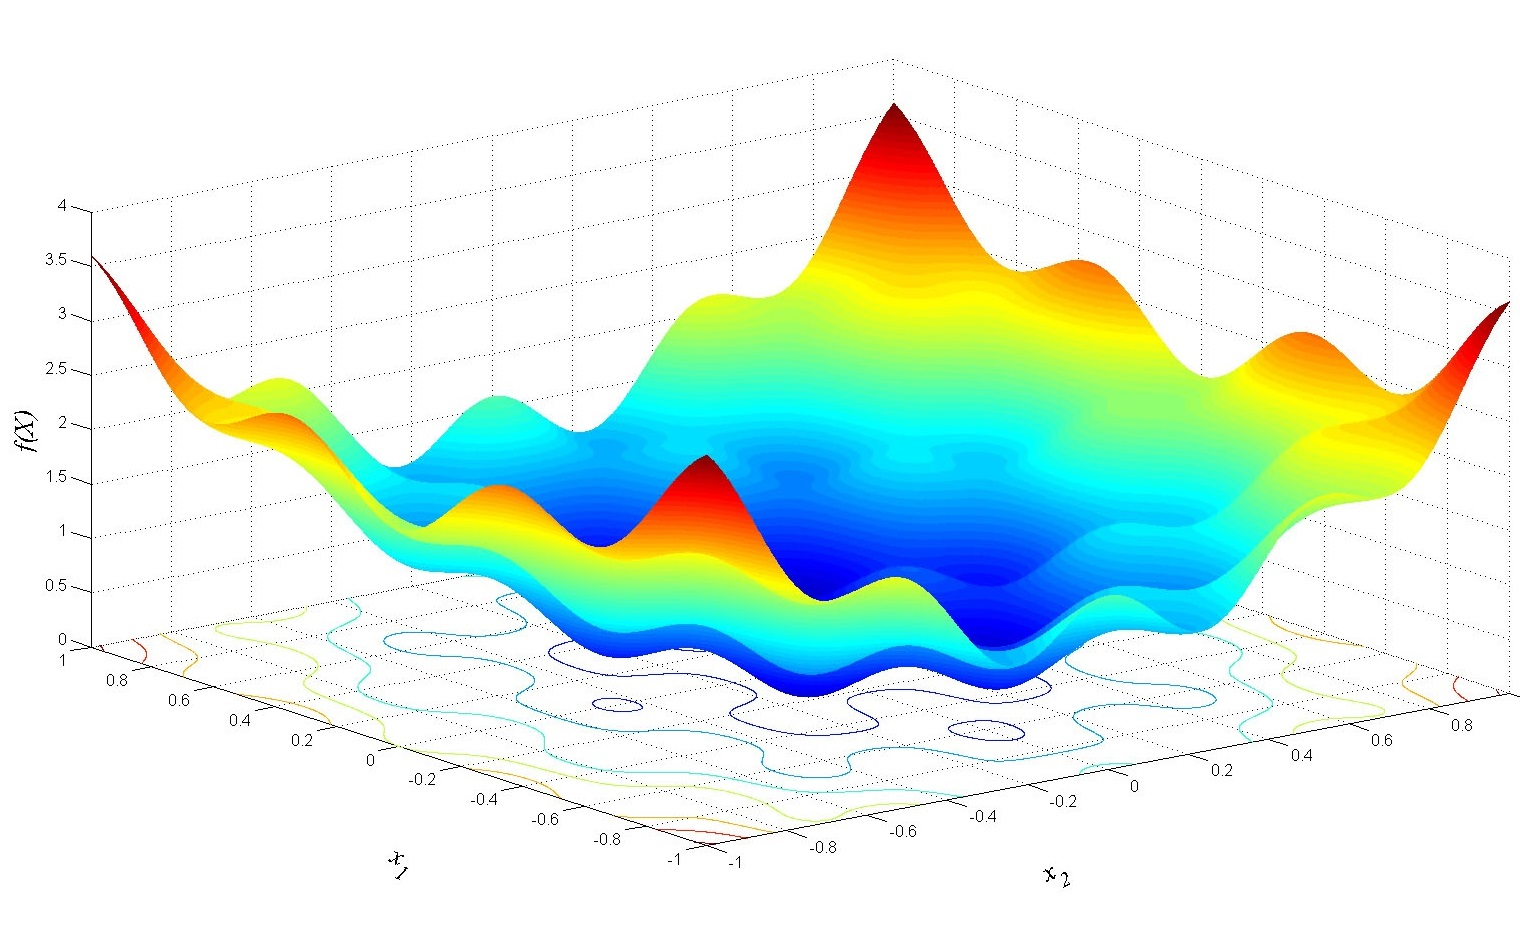
\includegraphics[width=0.4\textwidth]{img/sgd/non_convex_function.jpg}\\
Convex Function & Non-Convex Function
\end{tabular}
\end{figure}
\end{frame}

%%%%%%%%%%%%%%%%%%%%%%%%%%%%%%%%%%%%%%%%%%%%%%%%%%%%%%%%%%%%%%%%%%

\begin{frame}{Gradient Descent}
Gradient descent is often used in machine learning to \textbf{minimize a cost function}, usually also called \textit{objective} or \textit{loss} function and denoted $L(\cdot)$ or $J(\cdot)$.\\
\vspace{0.5cm}
The cost function depends on the model's parameters and is a proxy to evaluate model's performance. Generally speaking, in this framework minimizing the cost equals to maximizing the effectiveness of the model.

\end{frame}

%%%%%%%%%%%%%%%%%%%%%%%%%%%%%%%%%%%%%%%%%%%%%%%%%%%%%%%%%%%%%%%%%%

\begin{frame}{Stochastic Gradient Descent}
In principle, to perform a single update step you should run through all your training examples. This is known as \textbf{batch gradient descent}.\\
\vspace{0.5cm}
A different strategy is the one of \textbf{minibatch stochastic gradient descent}. In this case, only a small subset of the training dataset is considered at each update step.\\
\vspace{0.5cm}
In the extreme case in which only a random example of the training set is considered to perform the update step, we talk of \textbf{stochastic gradient descent}.

\end{frame}

%%%%%%%%%%%%%%%%%%%%%%%%%%%%%%%%%%%%%%%%%%%%%%%%%%%%%%%%%%%%%%%%%%

\begin{frame}{Learning Rate}
Choosing the the right \textbf{learning rate} $\bm{\alpha}$ is essential to correctly proceed towards the minimum. A step \textit{too small} could lead to an extremely \textit{slow} convergence. If the step is \textit{too big} the optimizer could \textit{overshoot} the minimum or even \textit{diverge}. 
\begin{figure}
\begin{tabular}{ccc}
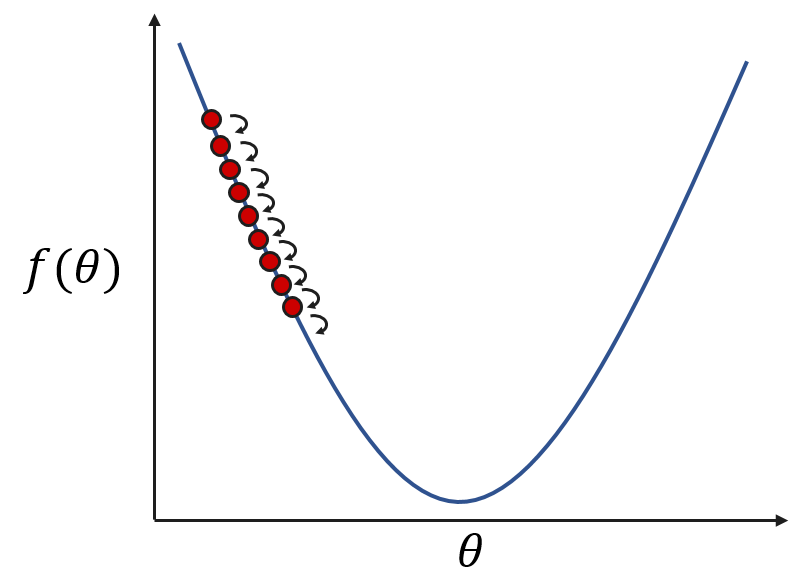
\includegraphics[width=0.35\textwidth]{img/sgd/lr_too_small.png} &
\quad &
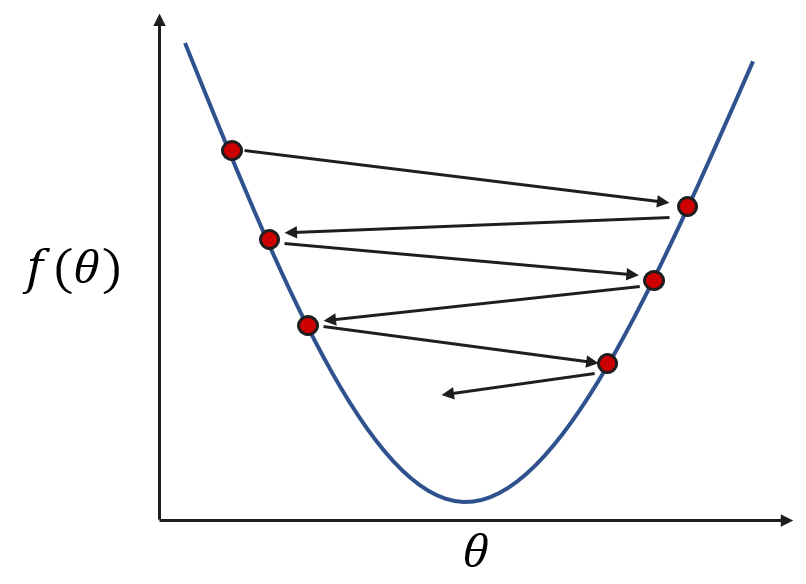
\includegraphics[width=0.35\textwidth]{img/sgd/lr_too_big.png}\\
Learning Rate too small & & Learning Rate too big
\end{tabular}
\end{figure}

\end{frame}

%%%%%%%%%%%%%%%%%%%%%%%%%%%%%%%%%%%%%%%%%%%%%%%%%%%%%%%%%%%%%%%%%%

\begin{frame}{Advanced Optimizers}
In practice, it's quite rare to see the procedure described above (so called \textbf{vanilla SGD}) used for optimization in the real-world.\\
\vspace{0.5cm}
Conversely, a number of cutting-edge optimizers  \cite{kingma2014adam,duchi2011adaptive,zeiler2012adadelta} are commonly used. However, these advanced optimization techniques are out of the scope of this short overview.
\end{frame}

%%%%%%%%%%%%%%%%%%%%%%%%%%%%%%%%%%%%%%%%%%%%%%%%%%%%%%%%%%%%%%%%%%
%%%%%%%%%%%%%%%%%%%%%%%%%%%%%%%%%%%%%%%%%%%%%%%%%%%%%%%%%%%%%%%%%%
%%%%%%%%%%%%%%%%%%%%%%%%%%%%%%%%%%%%%%%%%%%%%%%%%%%%%%%%%%%%%%%%%%

\section{Credits}
\begin{frame}[t, allowframebreaks]{Credits}
These slides heavily borrow from a number of awesome sources. I'm really grateful to all the people who take the time to share their knowledge on this subject with others.\\
\vspace{0.5cm}
In particular:
\begin{itemize}
\item Stanford CS231n Convolutional Neural Networks for Visual Recognition\\
\url{http://cs231n.stanford.edu/}
\item Stanford CS20SI TensorFlow for Deep Learning Research\\
\url{http://web.stanford.edu/class/cs20si/syllabus.html}
\item Deep Learning Book (GoodFellow, Bengio, Courville)\\
\url{http://www.deeplearningbook.org/}
\item Marc'Aurelio Ranzato, "Large-Scale Visual Recognition with Deep Learning"\\
\url{www.cs.toronto.edu/~ranzato/publications/ranzato_cvpr13.pdf}
\item Convolution arithmetic animations\\
\url{https://github.com/vdumoulin/conv_arithmetic}
\item Andrej Karphathy personal blog\\
\url{http://karpathy.github.io/}
\item WildML blog on AI, DL and NLP\\
\url{http://www.wildml.com/}
\item Michael Nielsen Deep Learning online book
\url{http://neuralnetworksanddeeplearning.com/}
\end{itemize}
\end{frame}

%%%%%%%%%%%%%%%%%%%%%%%%%%%%%%%%%%%%%%%%%%%%%%%%%%%%%%%%%%%%%%%%%%
%%%%%%%%%%%%%%%%%%%%%%%%%%%%%%%%%%%%%%%%%%%%%%%%%%%%%%%%%%%%%%%%%%
%%%%%%%%%%%%%%%%%%%%%%%%%%%%%%%%%%%%%%%%%%%%%%%%%%%%%%%%%%%%%%%%%%

\section{References}

\begin{frame}[t, allowframebreaks]
\frametitle{References}
\bibliographystyle{abbrv}
\bibliography{bibliography}
\end{frame}
\end{document}
\bgroup
\begin{frame}{Value function approximation by SGD}
\begin{itemize}
\item Goal: find parameter vector $\textbf{w}$ minimising mean-squared error between approximate value function $\hat{v}(s,\textbf{w})$ and true value function $v_{\pi}(s)$
\begin{equation*}
J(\textbf{w}) = \mathbb{E}_{\pi}[(v_{\pi}(S)-\hat{v}(S, \textbf{w}))^2]
\end{equation*}
\item Gradient descent finds a local minimum
\begin{align*}
\Delta\textbf{w} &= -\frac{1}{2}\alpha \nabla_{\textbf{w}}J(\textbf{w})\\
&= \alpha E_{\pi} [(v_{\pi}(S) - \hat{v}(S,\textbf{w}))\nabla_{\textbf{w}}\hat{v}(S,\textbf{w})]
\end{align*}
\item Stochastic gradient descent samples the gradient
\begin{equation*}
\Delta\textbf{w} = \alpha(v_{\pi}(S) - \hat{v}(S,\textbf{w}))\nabla_{\textbf{w}}\hat{v}(S,\textbf{w})
\end{equation*}
\item Expected update is equal to full gradient update
\end{itemize}
\end{frame}
\egroup
\bgroup
\begin{frame}{Feature vectors}
\begin{itemize}
\item Represent state by a feature vector
\begin{equation*}
\textbf{x}(S) = \left(\begin{array}{c}
\textbf{x}_1(S)\\
\vdots\\
\textbf{x}_n(S)
\end{array}
\right)
\end{equation*}
\item For example:
\begin{itemize}
\item Distance of robot from landmarks
\item Trends in the stock market
\item Piece and pawn configurations in chess
\end{itemize}
\end{itemize}
\end{frame}
\egroup
\bgroup
\begin{frame}{Linear value function approximation}
\begin{itemize}
\item Represent value function by a linear combination of features
\begin{equation*}
\hat{v}(S,\textbf{w}) = \textbf{x}(S)^T\textbf{w} = \sum_{j=1}^n\textbf{x}_j(S)\textbf{w}_j
\end{equation*}
\item Objective function is quadratic in parameters $\textbf{w}$
\begin{equation*}
J(\textbf{w}) = \mathbb{E}_{\pi}[(v_{\pi}(S) - \textbf{x}(S)^T\textbf{w})^2]
\end{equation*}
\item Stochastic gradient descent converges on global optimum
\item Update rule is particularly simple
\begin{align*}
\nabla_{\textbf{w}}\hat{v}(S,\textbf{w}) &= \textbf{x}(S)\\
\Delta w &= \alpha(v_{\pi}(S) - \hat{v}(S,\textbf{w}))\textbf{x}(S)
\end{align*}
Update = $stepsize \times prediction error \times feature value$
\end{itemize}
\end{frame}
\egroup
\bgroup
\begin{frame}{Table Lookup Features}
\begin{itemize}
\item Table lookup is a special case of linear value function approximation
\item Using table lookup features
\begin{equation*}
\textbf{x}^{table}(S)=\left(\begin{array}{c}
\textbf{1}(S=s_1)\\
\vdots\\
\textbf{1}(S=s_n)
\end{array}
\right)
\end{equation*}
\item Parameter vector $\textbf{w}$ gives value of each individual state
\begin{equation*}
\hat{v}(S, \textbf{w})=\left(\begin{array}{c}
\textbf{1}(S=s_1)\\
\vdots\\
\textbf{1}(S=s_n)
\end{array}\right)
\cdot
\left(\begin{array}{c}
\textbf{w}_1\\
\vdots\\
\textbf{w}_n
\end{array}\right)
\end{equation*}
\end{itemize}
\end{frame}
\egroup
\bgroup
\begin{frame}{Incremental prediction algorithms}
\begin{itemize}
\item Have assumed true value function $v_{\pi}(s)$ given by supervisor
\item But in RL there is no supervisor, only rewards
\item In practice, we substitute a \emph{target} for $v_{\pi}(s)$
\begin{itemize}
\item For MC, the target is the return $G_t$
\begin{equation*}
\Delta \textbf{w} = \alpha(\highlight{G_t} - \hat{v}(S_t, \textbf{w}))\nabla_{\textbf{w}}\hat{v}(S_t, \textbf{w})
\end{equation*}
\item For TD(0), the target is the TD target $R_{t+1} + \gamma \hat{v}(S_{t+1}, \textbf{w})$
\begin{equation*}
\Delta \textbf{w} = \alpha(\highlight{R_{t+1} + \gamma \hat{v}(S_{t+1}, \textbf{w})} - \hat{v}(S_t, \textbf{w}))\nabla_{\textbf{w}}\hat{v}(S_t, \textbf{w})
\end{equation*}


\end{itemize}
\end{itemize}
\end{frame}
\egroup
\bgroup
\begin{frame}{Monte-Carlo with value function approximation}
\begin{itemize}
\item Return $G_t$ is an unbiased, noisy sample of true value $v_{\pi}(S_t)$
\item Can therefore apply supervised learning to ``training data'':
\begin{equation*}
\left<S_1, G_1\right>,\left<S_2, G_2\right>,\ldots,\left<S_T, G_T\right>
\end{equation*}
\item For example, using \emph{linear Monte-Carlo policy evaluation}
\begin{align*}
\Delta \textbf{w} &= \alpha(\highlight{G_t}-\hat{v}(S_t, \textbf{w}))\nabla_{\textbf{w}}\hat{v}(S_t, \textbf{w})\\
&=\alpha(G_t-\hat{v}(S_t, \textbf{w}))\textbf{x}(S_t)
\end{align*}
\item Monte-Carlo evaluation converges to a local optimum
\item Even when using non-linear value function approximation
\end{itemize}
\end{frame}
\egroup
\bgroup
\begin{frame}{TD learning with value function approximation}
\begin{itemize}
\item The TD-target $R_{t+1} + \gamma \hat{v}(S_{t+1}, \textbf{w})$ is a \emph{biased} sample of true value $v_{\pi}(S_t)$
\item Can still apply supervised learning to ``training data'':
\begin{equation*}
\left<S_1, R_{2} + \gamma \hat{v}(S_{2}, \textbf{w})\right>,
\left<S_2, R_{3} + \gamma \hat{v}(S_{3}, \textbf{w})\right>,
\ldots,
\left<S_{T-1}, R_{T}\right>
\end{equation*}
%
\item Linear TD(0) update is
\begin{align*}
\Delta \textbf{w} &= \alpha(\highlight{R+\gamma \hat{v}(S^{\prime}, \textbf{w})} - \hat{v}(S, \textbf{w}))\nabla_{\textbf{w}}\hat{v}(S, \textbf{w})\\
&= \alpha \delta \textbf{x}(S)
\end{align*}
%
\item Linear TD(0) converges (close) to global optimum
\end{itemize}
\end{frame}
\egroup
\bgroup
\begin{frame}{Control with value function approximation}
\begin{figure}
\centering
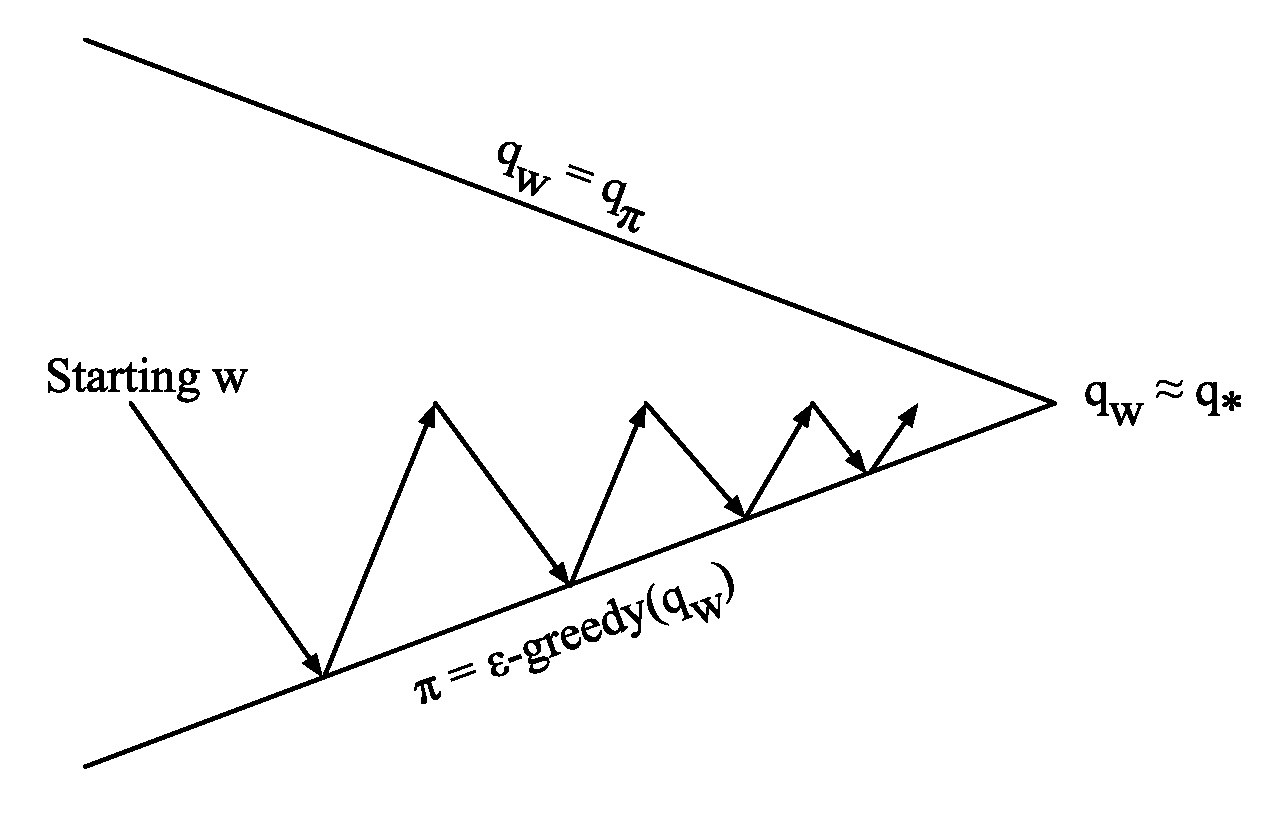
\includegraphics[width=0.6\textwidth]{img/vfa_control}
\end{figure}
\highlight{Policy evaluation Approximate} policy evaluation, $\hat{q}(\cdot, cdot, \textbf{w}) \approx q_{\pi}$\\
\highlight{Policy improvement} $\epsilon$-greedy policy improvement
\end{frame}
\egroup
\bgroup
\begin{frame}{Action-value function approximation}
\begin{itemize}
\item Approximate the action-value function
\begin{equation*}
\hat{q}(S,A,\textbf{w})\approx q_{\pi}(S,A)
\end{equation*}
%
\item Minimise mean-squared error between approximate
action-value function $\hat{q}(S,A,\textbf{w})$ and true action-value function $q_{\pi}(S, A)$
\begin{equation*}
J(\textbf{w})=\mathbb{E}_{\pi}[(q_{\pi}(S, A)-\hat{q}(S,A,\textbf{w}))^2]
\end{equation*}
%
\item Use stochastic gradient descent to nd a local minimum
\begin{align*}
-\frac{1}{2}\nabla_{\textbf{w}}J(\textbf{w})&=(q_{\pi}(S, A)-\hat{q}(S,A,\textbf{w}))\nabla_{\textbf{w}}\hat{q}(S,A,\textbf{w})\\
\Delta \textbf{w} &= \alpha(q_{\pi}(S, A)-\hat{q}(S,A,\textbf{w}))\nabla_{\textbf{w}}\hat{q}(S,A,\textbf{w})
\end{align*}
%
\end{itemize}
\end{frame}
\egroup
\bgroup
\begin{frame}{Linear action-value function approximation}
\begin{itemize}
\item Represent state \emph{and} action by a \emph{feature} vector
\begin{equation*}
\textbf{x}(S,A)=\left(\begin{array}{c}
\textbf{x}_1(S,A)\\
\vdots\\
\textbf{x}_n(S,A)
\end{array}\right)
\end{equation*}
%
\item Represent action-value function by linear combination of features
\begin{equation*}
\hat{q}(S, A, \textbf{w}) = \textbf{x}(S,A)^T\textbf{w}=\sum_{j=1}^n\textbf{x}_j(S,A)\textbf{w}_j
\end{equation*}
%
\item Stochastic gradient descent update
\begin{align*}
\nabla_w\hat{q}(S,A,\textbf{w})&=\textbf{x}(S,A)\\	
\Delta \textbf{w} &= \alpha(q_{\pi}(S,A)-\hat{q}(S,A,\textbf{w}))\textbf{x}(S,A)
\end{align*}
\end{itemize}
\end{frame}
\egroup
\bgroup
\begin{frame}{Incremental control algorithms}
\begin{itemize}
\item Like prediction, we must substitute a target for $q_{\pi}(S,A)$
\begin{itemize}
\item For MC, the target is the return $G_t$
\begin{equation*}
\Delta \textbf{w} = \alpha(\highlight{G_t} - \hat{q}(S_t, A_t, \textbf{w}))\nabla_{\textbf{w}}\hat{q}(S_t,A_t, \textbf{w})
\end{equation*}
%
\item For TD(0), the target is the TD target $R_{t+1} + \gamma Q(S_{t+1}, A_{t+1})$
\begin{equation*}
\Delta \textbf{w} = \alpha(\highlight{R_{t+1} + \gamma \hat{q}(S_{t+1}, A_{t+1}, \textbf{w})} - \hat{q}(S_t, A_t, \textbf{w}))\nabla_{\textbf{w}}\hat{q}(S_t,A_t, \textbf{w})
\end{equation*}
\end{itemize}
\end{itemize}
\end{frame}
\egroup
\bgroup
\begin{frame}{Linear SARSA in mountain car}
\centering
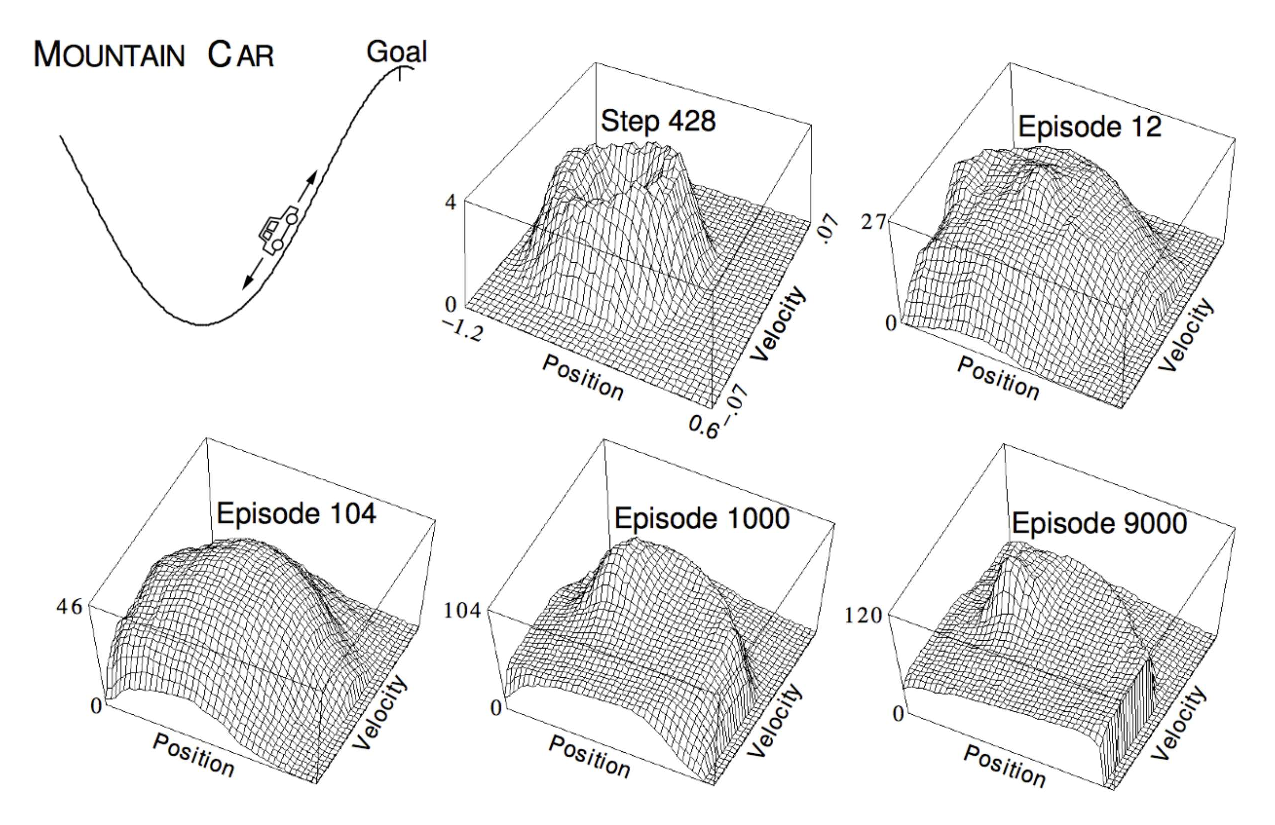
\includegraphics[width=0.8\textwidth]{img/mountain_car}
\end{frame}
\egroup
\bgroup
\begin{frame}{Convergence of prediction algorithms}
\begin{table}
\begin{tabular}{ccccc}
\hline
On/Off Policy & Algorithm & Table Lookup & Linear & Non-Linear\\ \hline
\multirow{2}{*}{On-policy} & MC & \cmark & \cmark & \cmark \\
& TD(0) & \cmark & \cmark & \xmark\\ \hline
\multirow{2}{*}{Off-policy} & MC & \cmark & \cmark & \cmark \\
& TD(0) & \cmark & \xmark & \xmark\\ \hline

\end{tabular}
\end{table}
\end{frame}
\egroup
\bgroup
\begin{frame}{Convergence of prediction algorithms}
\begin{table}
\begin{tabular}{cccc}
\hline
Algorithm & Table Lookup & Linear & Non-Linear\\ \hline
Monte-Carlo Control & \cmark & (\cmark) & \xmark \\
Sarsa & \cmark & (\cmark) & \xmark \\
Q-learning & \cmark & \xmark & \xmark \\\hline
\end{tabular}
\end{table}
(\cmark) = chatters around near-optimal value function
\end{frame}
\egroup

\section{Batch methods}
\bgroup
\begin{frame}{Batch reinforcement learning}
\begin{itemize}
\item Gradient descent is simple and appealing
\item But it is not sample efficient
\item Batch methods seek to find the best fitting value function
\item Given the agent's experience (``training data'')
\end{itemize}
\end{frame}
\egroup
\bgroup
\begin{frame}{Least squares prediction}
\begin{itemize}
\item Given value function approximation $\hat{v}(s,\textbf{w})\approx v_{\pi}(s)$
\item And \emph{experience} $\mathcal{D}$ of $\left<state,value\right>$ pairs
\begin{equation*}
\mathcal{D}=\{\left<s_1,v_1^{\pi}\right>,
\left<s_2,v_2^{\pi}\right>,
\ldots,
\left<s_T,v_T^{\pi}\right>\}
\end{equation*}
%
\item Which parameters $\textbf{w}$ give the best fitting value function $\hat{v}(s, \textbf{w})$?
\item \highlight{Least squares} algorithms find parameter vector $\textbf{w}$ minimising sum-squared error between $\hat{v}(s_t,\textbf{w})$ and target values $v_t^{\pi}$,
\begin{align*}
LS(\textbf{w})&=\sum_{t=1}^T(v_t^{\pi} - \hat{v}(s_t,\textbf{w}))^2\\
&=\mathbb{E}_{\mathcal{D}}[(v^{\pi} - \hat{v}(s,\textbf{w}))^2]
\end{align*}
\end{itemize}
\end{frame}
\egroup
\bgroup
\begin{frame}{Stochastic gradient descent with experience replay}
Given experience consisting of $\left<state,value\right>$ pairs
\begin{equation*}
\mathcal{D}=\{\left<s_1,v_1^{\pi}\right>,
\left<s_2,v_2^{\pi}\right>,
\ldots,
\left<s_T,v_T^{\pi}\right>\}
\end{equation*}
Repeat:
\begin{enumerate}
\item Sample state, value from experience
\begin{equation*}
\left<s, v^{\pi}\right>\sim\mathcal{D}
\end{equation*}
\item Apply stochastic gradient descent update
\begin{equation*}
\Delta \textbf{w}=\alpha(v^{\pi}-\hat{v}(s,\textbf{w}))\nabla_{\textbf{w}}\hat{v}(s, \textbf{w})
\end{equation*}
\end{enumerate}
\onslide<2->{
Converges to least squares solution
\begin{equation*}
\textbf{w}^{\pi}=\argmin_{\textbf{w}}LS(\textbf{w})
\end{equation*}}
\end{frame}
\egroup
\bgroup
\begin{frame}{Experience replay in deep Q-networks (DQN)}
DQN uses \highlight{experience replay} and \highlight{fixed Q-targets}
\begin{itemize}
\item Take action $a_t$ according to $\epsilon$-greedy policy
\item Store transition $(s_t, a_t, r_{t+1}, s_{t+1})$ in replay memory $\mathcal{D}$
\item Sample random mini-batch of transitions $(s, a, r, s^{\prime})$ from $\mathcal{D}$
\item Compute Q-learning targets w.r.t. old, fixed parameters $w^{-}$
\item Optimise MSE between Q-network and Q-learning targets
\begin{equation*}
\mathcal{L}_i(w_i)=\mathbb{E}_{s,a,r,s^{\prime}\sim\mathcal{D}_i}\left[\left(r + \gamma \max_{a^{\prime}}Q(s^{\prime}, a^{\prime};w_i^{-}) - Q(s, a, w_i)\right)^2\right]
\end{equation*}
\item Using variant of stochastic gradient descent
\end{itemize}
\end{frame}
\egroup
\bgroup
\begin{frame}{DQN in Atari}
\begin{itemize}
\item End-to-end learning of values $Q(s, a)$ from pixels $s$
\item Input state $s$ is stack of raw pixels from last 4 frames
\item Output is $Q(s, a)$ for 18 joystick/button positions
\item Reward is change in score for that step
\end{itemize}
\begin{figure}
\centering
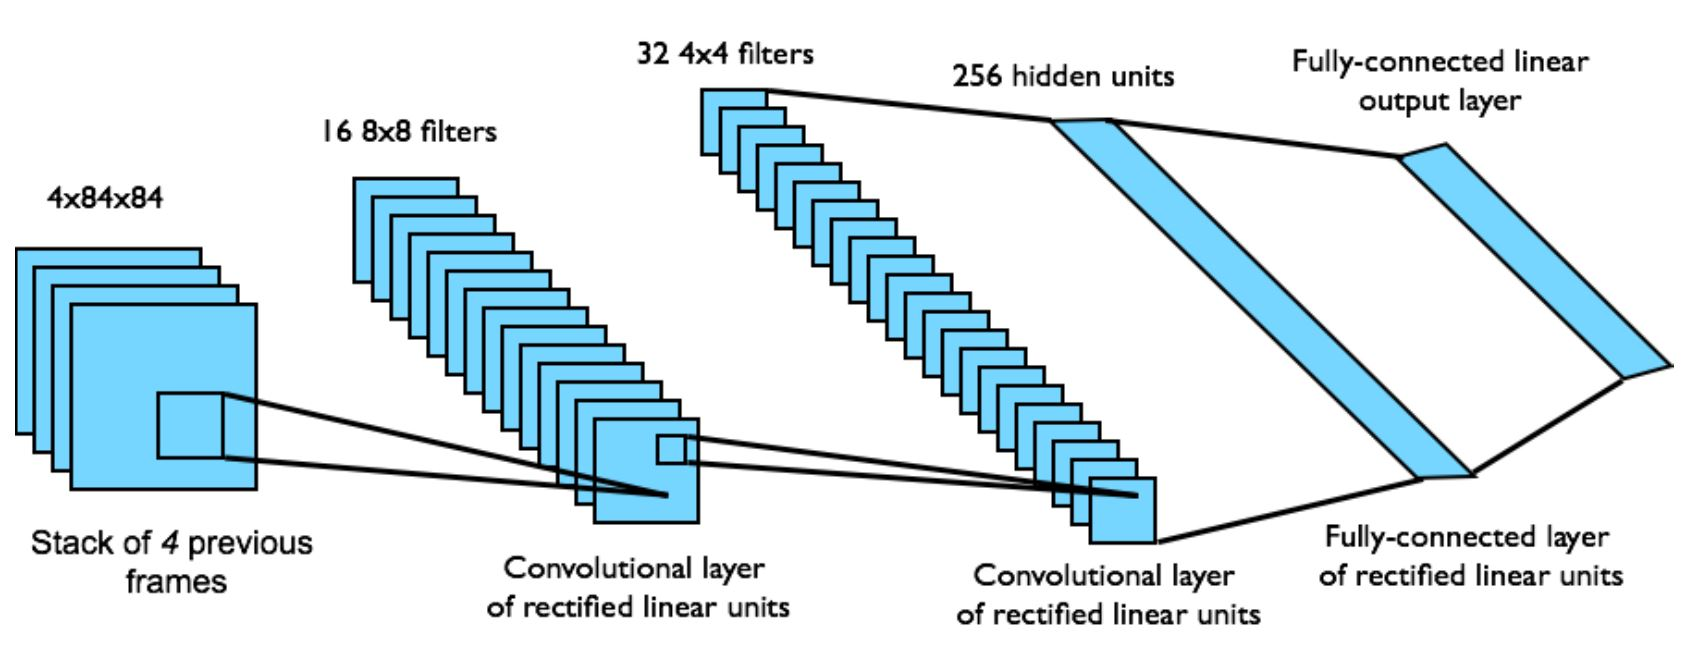
\includegraphics[width=0.8\textwidth]{img/dqn.jpg}
\end{figure}
\end{frame}
\egroup
\bgroup
\begin{frame}{DQN results in Atari}
\centering
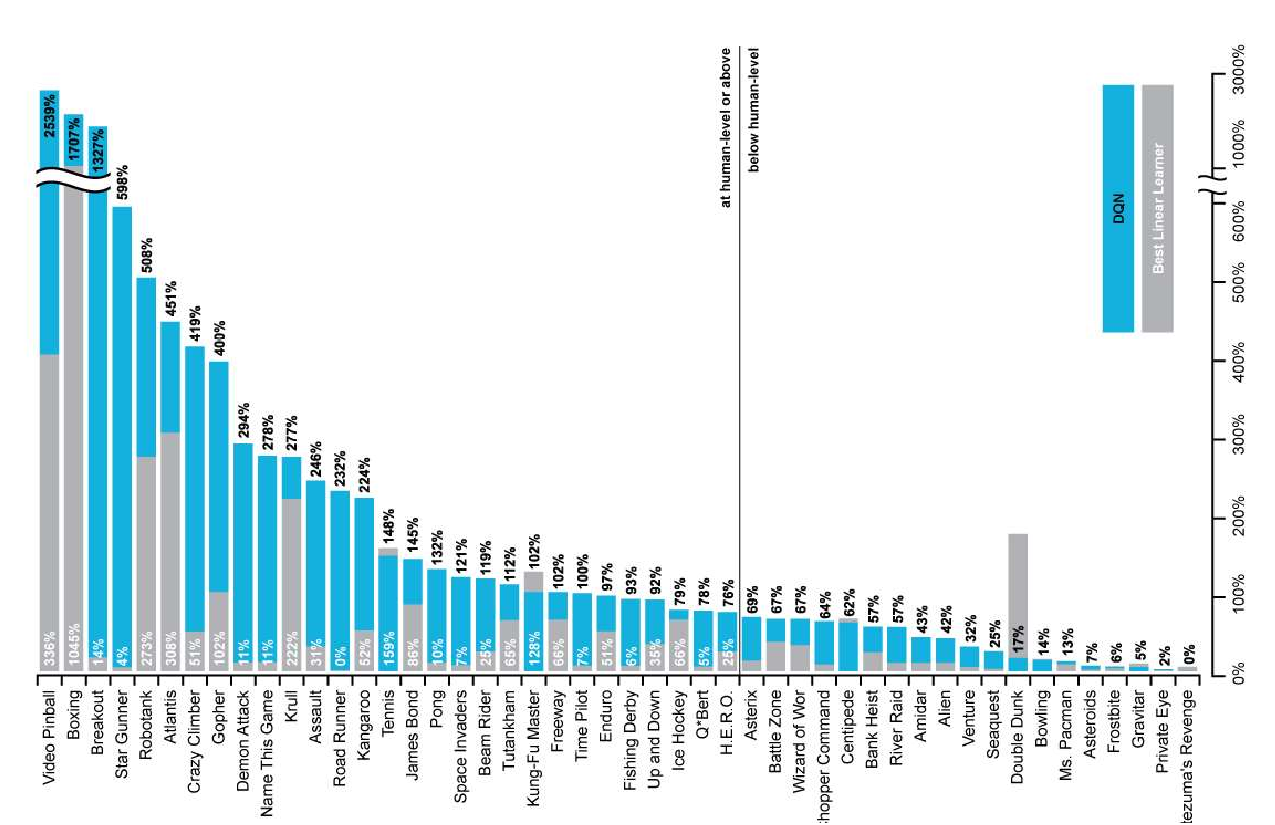
\includegraphics[width=0.85\textwidth]{img/dqn_results.pdf}
\end{frame}
\egroup


\end{document}